\documentclass{beamer}

\usepackage{array}
\usepackage{graphics}
\usepackage{tikz}
\usepackage{siunitx}
\usepackage{xcolor}
\usepackage{systeme}
\usepackage{bm}
\usepackage{enumerate}
\usepackage{pgfplots}

\usetikzlibrary{fit, shapes, arrows, positioning}
\pgfplotsset{compat=1.16} % it's recommended to use an explicit version number


\author{Daniel Lisser und Cedric Geissmann}
\title{Präsentation mit {\LaTeX} Beamer\\ und Geogebra}
\date{07. Dezember 2020}

\setbeamertemplate{navigation symbols}{}

\begin{document}

\begin{frame}
    \titlepage
\end{frame}

\begin{frame}[c]
    \frametitle{Wieso mit {\LaTeX} präsentieren?}
\begin{itemize}
    \item Schnell und einfach
    \item Konsistentes Design
    \item Super flexibel
    \item Saubere und schöne Präsentationen
    \item Textbasiert
\end{itemize}
\end{frame}

\begin{frame}[c]
    \frametitle{Beispiele}
    \begin{center}
        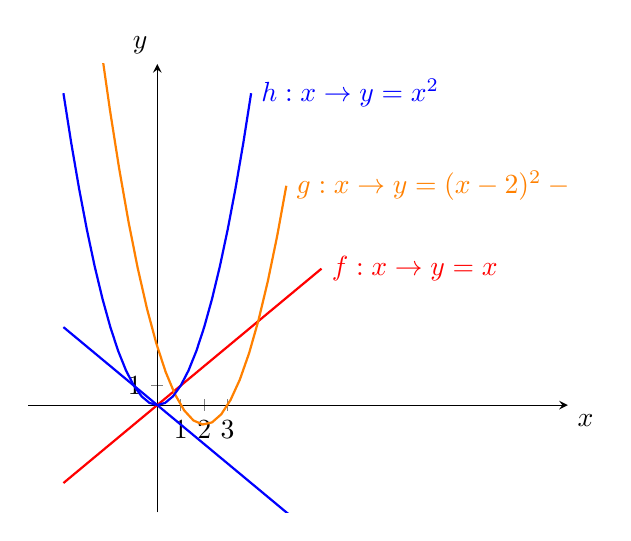
\begin{tikzpicture}
            \begin{axis}[
                axis x line=center,
                axis y line=center,
                xtick={1,2,3},
                ytick={1},
                xlabel={$x$},
                ylabel={$y$},
                xlabel style={below right},
                ylabel style={above left},
                xmin=-5.5,
                xmax=17.5,
                ymin=-5.5,
                ymax=17.5]
                \addplot[thick, blue, domain=-4:7] {-x} node[right] {$f: x
                    \rightarrow y = x$};
                \addplot[thick, red, domain=-4:7] {x} node[right] {$f: x
                    \rightarrow y = x$};
                \addplot[thick, orange, domain=-4:5.5] {(x-2)^2-1} node[right]
                    {$g: x \rightarrow y = (x-2)^2-1$};
                \addplot[thick, blue, domain=-4:4] {x^2} node[right] {$h: x
                    \rightarrow y = x^2$};
            \end{axis}
        \end{tikzpicture}
    \end{center}
\end{frame}

\begin{frame}[c]
    \frametitle{Geogebra}
    \framesubtitle{Direkt exportiert}
    \centering
    \definecolor{ffqqqq}{rgb}{1,0,0}
    \definecolor{qqqqff}{rgb}{0,0,1}
    \begin{tikzpicture}[scale=0.7,line cap=round,line join=round,>=triangle 45,x=1cm,y=1cm]
        \begin{axis}[
            x=1cm,y=1cm,
            axis lines=middle,
            ymajorgrids=true,
            xmajorgrids=true,
            xmin=-7.75142857142857,
            xmax=4.905714285714287,
            ymin=-4.481428571428576,
            ymax=4.2614285714285725,
            xtick={-7.5,-7,...,4.5},
            ytick={-4,-3.5,...,4},]
            \clip(-7.75142857142857,-4.481428571428576) rectangle (4.905714285714287,4.2614285714285725);
            \draw [line width=2pt,color=qqqqff,domain=-7.75142857142857:4.905714285714287]
                plot(\x,{(-1--0.5*\x)/1});
            \draw [line width=2pt,color=ffqqqq,domain=-7.75142857142857:4.905714285714287] plot(\x,{(--2-1*\x)/1});
            \begin{scriptsize}
                \draw[color=qqqqff] (-6.7228571428571415,-4.363571428571433) node {$f$};
                \draw[color=ffqqqq] (-2.10142857142857,4.229285714285715) node {$g$};
            \end{scriptsize}
        \end{axis}
    \end{tikzpicture}
\end{frame}

\begin{frame}[c]
    \frametitle{Geogebra}
    \framesubtitle{Kleine Manipulationen}
    \centering
    \definecolor{ffqqqq}{rgb}{1,0,0}
    \definecolor{qqqqff}{rgb}{0,0,1}
    \begin{tikzpicture}[scale=0.7,line cap=round,line join=round,>=triangle 45,x=1cm,y=1cm]
        \begin{axis}[
            x=1cm,y=1cm,
            axis lines=middle,
            ymajorgrids=true,
            xmajorgrids=true,
            xmin=-7.75142857142857,
            xmax=4.905714285714287,
            ymin=-4.481428571428576,
            ymax=4.2614285714285725,
            xtick={-7,-6,...,4},
            ytick={-4,-3,...,4},]
            \draw [line width=2pt,color=qqqqff,domain=-7.75142857142857:4.905714285714287]
                plot(\x,{(-1--0.5*\x)/1});
            \only<2->{%
                \draw [line width=2pt, color=ffqqqq,
                    domain=-7.75142857142857:4.905714285714287]
                    plot(\x,{(--2-1*\x)/1});
            }
            \begin{scriptsize}
            \only<3-4>{%
                \draw[color=qqqqff] (-6.7228571428571415,-4.363571428571433)
                    node[above right=0cm and 1.5cm] {$f: x \rightarrow y =
                    \frac{1}{2}\cdot x-1$};
            }
            \only<4->{%
                \draw[color=ffqqqq] (-2.10142857142857,4.229285714285715)
                    node[below left] {$g: x \rightarrow y = -x +2$};
            }
            \only<5->{%
                \draw[ultra thick, orange] (2, 0) circle (0.5cm);
            }
            \end{scriptsize}
        \end{axis}
    \end{tikzpicture}
\end{frame}

\begin{frame}[c]
    \frametitle{Nullstellen bestimmen}
    \huge
    \[\textcolor{green}{a}\cdot (x - \textcolor{blue}{u})^2 +
    \textcolor{red}{v} = 0 \]
    \pause
    \[x_{1,2} = \textcolor{blue}{u} \pm
    \sqrt{\frac{\textcolor{red}{-v}}{\textcolor{green}{a}}} \]
\end{frame}

\newcommand{\ca}{\ensuremath{\textcolor{green}{a}}}
\newcommand{\cb}{\ensuremath{\textcolor{blue}{b}}}
\newcommand{\cc}{\ensuremath{\textcolor{red}{c}}}

\begin{frame}[c]
    \frametitle{Nullstellen bestimmen}
    \framesubtitle{Allgemein}
    \huge
    \[ \ca\cdot x^2 + \cb\cdot x + \cc = 0 \]
    \pause
    \vspace{1cm}
    \[ x_{1,2} = \frac{-\cb \pm \sqrt{\cb^2 - 4 \cdot \ca \cdot \cc}}{2\cdot \ca}
    \]
\end{frame}

\begin{frame}[c]
    \frametitle{Tetris}
    \framesubtitle{Tolle Einstiege in die Lektion}
    \begin{center}
        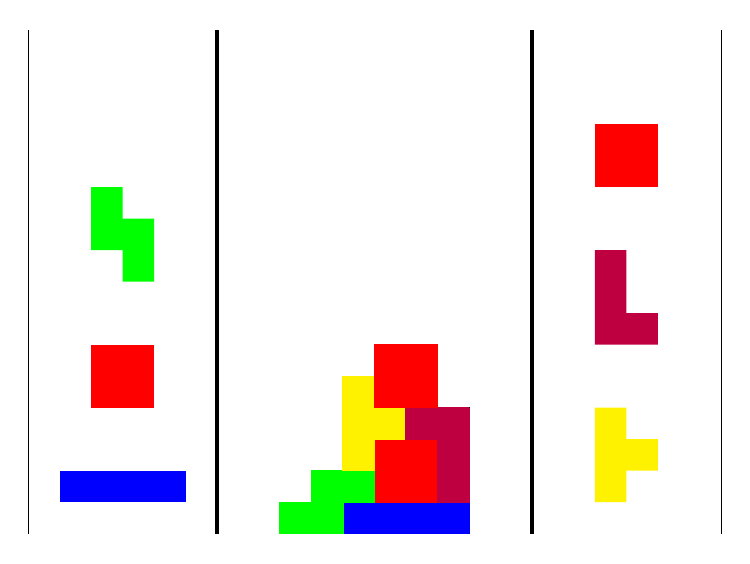
\begin{tikzpicture}[scale=0.4]
            \draw[line width=.1mm] (0, 0) -- ++(0, 16);
            \draw[line width=.5mm] (6, 0) -- ++(0, 16);
            \draw[line width=.5mm] (16, 0) -- ++(0, 16);
            \draw[line width=.1mm] (22, 0) -- ++(0, 16);

            \fill[blue] (1, 1) rectangle ++(4, 1);
            \fill[red] (2, 4) rectangle ++(2, 2);
            \fill[green] (4, 8) -- ++(0, 2) -- ++(-1, 0) -- ++(0, 1) -- ++(-1, 0) --
                ++(0, -2) -- ++(1, 0) -- ++(0, -1) -- ++(1, 0);

            \fill[yellow] (18, 1) -- ++(1, 0) -- ++(0, 1) -- ++(1, 0) -- ++(0, 1) --
                ++(-1, 0) -- ++(0, 1) -- ++(-1, 0) -- ++(0, -3);

            \fill[purple] (18, 6) -- ++(2, 0) -- ++(0, 1) -- ++(-1, 0) -- ++(0, 2) --
                ++(-1, 0) -- ++(0, -3);

            \fill[red] (18, 11) rectangle ++(2, 2);


            \draw[line width=0.1mm] (8,0) --
                ++(0, 1) --
                ++(1, 0) --
                ++(0, 1) --
                ++(1, 0) --
                ++(0, 3) --
                ++(1, 0) --
                ++(0, 1) --
                ++(2, 0) --
                ++(0, -2) --
                ++(1, 0) --
                ++(0, -4) --
                (8, 0);

            \pause

            \filldraw[blue] (10, 0) rectangle ++(4, 1);
            \pause
            \filldraw[red] (11, 1) rectangle ++(2, 2);
            \pause
            \begin{scope}[rotate=90, shift={(2,-11)}]
                \filldraw[green] (0, 0) -- ++(0, 2) -- ++(-1, 0) -- ++(0, 1) -- ++(-1, 0) --
                    ++(0, -2) -- ++(1, 0) -- ++(0, -1) -- ++(1, 0);
            \end{scope}
            \pause
            \filldraw[yellow] (10, 2) -- ++(1, 0) -- ++(0, 1) -- ++(1, 0) -- ++(0, 1) --
                ++(-1, 0) -- ++(0, 1) -- ++(-1, 0) -- ++(0, -3);
            \pause
            \begin{scope}[rotate=180, shift={(-14,-4)}]
            \filldraw[purple] (0, 0) -- ++(2, 0) -- ++(0, 1) -- ++(-1, 0) -- ++(0, 2) --
                ++(-1, 0) -- ++(0, -3);
            \end{scope}
            \pause
            \filldraw[red] (11, 4) rectangle ++(2, 2);

        \end{tikzpicture}
    \end{center}
\end{frame}

\end{document}
